\documentclass[a4j]{jarticle}
\usepackage[dvipdfmx]{graphicx}
\usepackage{amsmath,amssymb,ascmac}
\usepackage{bm}
\usepackage{algorithm,algorithmic}
\usepackage{listings,plistings}
% 行範囲の終端で、読み込んだコードの残りだけを読み飛ばす。
\makeatletter
\long\def\study@EndInputListing#1\empty{}
\let\study@InputListing\lst@InputListing
\def\lst@InputListing#1{%
  \begingroup
  \let\lst@EndProcessListing\study@EndInputListing
  \study@InputListing{#1}%
  \endgroup
}
\makeatother
\lstset{%
  language={C},
  basicstyle={\small},%
  identifierstyle={\small},%
  commentstyle={\small\itshape},%
  keywordstyle={\small\bfseries},%
  ndkeywordstyle={\small},%
  stringstyle={\small\ttfamily},
  frame={tb},
  breaklines=true,
  columns=[l]{fullflexible},%
  numbers=left,%
  xrightmargin=0zw,%
  xleftmargin=3zw,%
  numberstyle={\scriptsize},%
  stepnumber=1,
  numbersep=1zw,%
  lineskip=-0.5ex%
}
\renewcommand{\lstlistingname}{コード}
\renewcommand{\lstlistlistingname}{コード目次}

%
% 以後をレポート課題ごとに書き換える。
%

\usepackage{url}

\newcommand{\toprule}{\hline}
\newcommand{\midrule}{\hline}
\newcommand{\bottomrule}{\hline}

\begin{document}

\begin{titlepage}
    \centering
    \vspace*{2cm}  % 上からの余白調整
    
    {\Huge \textbf{月3, 4 火3, 4 数理工学実験}}\\[1.5cm]
    
    {\huge 実験テーマ: 3 高速フーリエ変換}\\[2cm]
    
    
    {\Large 
    実験の実施年月日: 2026年11月9日 \\[1cm]
    実験の実施場所: 京都大学 工学部総合校舎 \\[1cm]
    レポートの提出年月日: \today \\[1cm]
    氏名: 井上 慧人 \\[1cm]
    所属: 工学部 情報学科 2年\\[1cm]
    学生番号: 1029374191 \\[0.5cm]
    }
    
    \vfill % 下部に余白を押しやる
    
\end{titlepage}

% 2ページ目以降の本文
\newpage


\begin{abstract}
関数の零点や関数値が小さくなる点を求める方法をPythonで実装し、それぞれの結果を比較した。零点探索では、二分法とニュートン法のどちらでも、$-3$、$-1$、$2$に近い値が得られた。最適化では、最急降下法とニュートン法でほぼ同じ点に到達したが、更新回数には違いがあった。課題4ではそれぞれ31回と6回、課題5では791回と5回であり、今回はニュートン法の方が少ない更新で解を求められた。このことから、進む方向の決め方によって、解に到達するまでの更新回数が大きく変わることが分かった。また、課題6では制約のある最適化問題について調べ、課題6-4で求めた数値解が解析解と一致することを確認した。
\end{abstract}


\section{はじめに}
零点探索と最適化の反復法を実装し、初期値、ステップサイズなどが収束に与える影響を調べる。問題設定と手法は教材に従う。実装コードと保存結果は提出ファイルの中に含まれる。

\section{原理・方法の詳細}
\subsection{零点探索}


\clearpage
\section{実験方法・結果・考察}
\label{sec:experiment}
\subsection{共通の実験条件}
\paragraph{実装・再現方法}
零点探索および降下法の共通処理は\texttt{utils\_math.py}に、課題の関数は\texttt{kadai*.py}に実装した。出力は各\texttt{kadai*.txt}に保存した。
本稿作成時の再検証には、以下の環境を使用した。
\begin{itemize}
  \item OS：macOS 26.3
  \item アーキテクチャ：arm64
  \item Python：3.9.6
  \item NumPy：2.0.2
\end{itemize}

\paragraph{終了条件と反復上限}
\begin{itemize}
  \item 課題1の終了条件：
\end{itemize}

\subsection{問題1：ギブズ現象}
\subsubsection{問題(1-a)}
\begin{itembox}[l]{問題1}
次の2つの周期関数について、以下の問いに答えよ。
\[
  \begin{aligned}
    \mathrm{A}:\quad & x(t)=t-[t],\\
    \mathrm{B}:\quad & x(t)=\left|\cos\left(\frac{\pi}{2}t\right)\right|.
  \end{aligned}
\]
ただし、$[t]$はガウス記号であり、$n$を整数として$t$が$n\le t<n+1$を満たすとき、$[t]=n$とする。
\begin{enumerate}
  \item[(a)] 上のA、Bの周期関数をフーリエ級数展開するときの$k$次のフーリエ係数$a_k$および$b_k$
  \[
    \begin{aligned}
      a_k&=\frac{2}{T}\int_{-T/2}^{T/2}x(t)\cos\left(\frac{2\pi k}{T}t\right)\,dt,\\
      b_k&=\frac{2}{T}\int_{-T/2}^{T/2}x(t)\sin\left(\frac{2\pi k}{T}t\right)\,dt
    \end{aligned}
  \]
  を求めよ。ただし、$T$は$x(t)$の基本周期である。
\end{enumerate}
\end{itembox}

\subsubsection{実験方法(1-a)}
式変形を行い、結果を示す。

\subsubsection{結果(1-a)}
まずは基本周期を求める。$x_A(t)=t-[t]$, $x_B(t)=\left|\cos\left(\frac{\pi}{2}t\right)\right|$と置く。$[t]$ はガウス記号より、

\[
x_A(t+1)=(t+1)-[t+1]=t-[t]=x_A(t).
\]

また、$x_A(0)=0$ であり、$0<t<1$ では $[t]=0$ なので $x_A(t)=t>0$ である。よって $1$ より小さい正の周期は存在せず、$x_A(t)$の基本周期は \textbf{$T_A=1$} となる。Bについては、$t$ を $2$ 増やすと、コサインの角度が $\pi$ 増えて符号が反転する。よって、

\[
\begin{aligned}
x_B(t+2)
&=\left|\cos\left(\frac{\pi}{2}t+\pi\right)\right|\\
&=\left|-\cos\left(\frac{\pi}{2}t\right)\right|\\
&=x_B(t).
\end{aligned}
\]

また、$x_B(0)=1$ であり、$0<t<2$ では角度 $\frac{\pi}{2}t$ が $0$ と $\pi$ の間にあるので $x_B(t)<1$ である。よって $2$ より小さい正の周期は存在せず、基本周期は \textbf{$T_B=2$} となる。

$T_A=1$ なので、積分区間は $[-\frac12,\frac12]$ となり、その区間で$x_A(t)$は以下のように書ける。

\[
x_A(t)=
\begin{cases}
t+1 & \left(-\dfrac12\le t<0\right),\\[4pt]
t & \left(0\le t\le\dfrac12\right).
\end{cases}
\]

以下、$k\ge 1$ とし、置換積分を $t=-u$ と置くと、

\[
\begin{aligned}
a_k
&=2\int_{-1/2}^{0}(t+1)\cos(2\pi kt)\,dt
  +2\int_0^{1/2}t\cos(2\pi kt)\,dt\\
&=2\int_0^{1/2}(1-u)\cos(2\pi ku)\,du
  +2\int_0^{1/2}u\cos(2\pi ku)\,du\\
&=2\int_0^{1/2}\cos(2\pi ku)\,du\\
&=2\left[\frac{\sin(2\pi ku)}{2\pi k}\right]_0^{1/2}\\
&=\frac{\sin(k\pi)}{\pi k}=0.
\end{aligned}
\]


\[
\begin{aligned}
b_k
&=2\int_{-1/2}^{0}(t+1)\sin(2\pi kt)\,dt
  +2\int_0^{1/2}t\sin(2\pi kt)\,dt\\
&=-2\int_0^{1/2}(1-u)\sin(2\pi ku)\,du
  +2\int_0^{1/2}u\sin(2\pi ku)\,du\\
&=2\int_0^{1/2}(2u-1)\sin(2\pi ku)\,du\\
&=2\left[
  -\frac{(2u-1)\cos(2\pi ku)}{2\pi k}
  +\frac{2\sin(2\pi ku)}{(2\pi k)^2}
  \right]_0^{1/2}\\
&=2\left(0-\frac{1}{2\pi k}\right)
=-\frac{1}{\pi k}.
\end{aligned}
\]

\[
\frac{a_0}{2}
=\int_{-1/2}^{0}(t+1)\,dt+\int_0^{1/2}t\,dt
=\frac38+\frac18=\frac12.
\]

Bについては、$T_B=2$ なので、積分区間は $[-1,1]$ である。この区間では

\[
-\frac{\pi}{2}\le \frac{\pi}{2}t\le \frac{\pi}{2}
\]

が成り立つので、 $x_B(t)=\cos(\frac{\pi}{2}t)$ と書ける。

$k\ge 1$ とすると

\[
\begin{aligned}
a_k
&=\int_{-1}^{1}\cos\left(\frac{\pi}{2}t\right)\cos(k\pi t)\,dt\\
&=2\int_0^1\cos\left(\frac{\pi}{2}t\right)\cos(k\pi t)\,dt\\
&=\int_0^1\left[
\cos\left(\left(k-\frac12\right)\pi t\right)
+\cos\left(\left(k+\frac12\right)\pi t\right)
\right]\,dt\\
&=\left[
\frac{\sin\left(\left(k-\frac12\right)\pi t\right)}{\left(k-\frac12\right)\pi}
+\frac{\sin\left(\left(k+\frac12\right)\pi t\right)}{\left(k+\frac12\right)\pi}
\right]_0^1\\
&=\frac{(-1)^{k+1}}{\left(k-\frac12\right)\pi}
+\frac{(-1)^k}{\left(k+\frac12\right)\pi}\\
&=\frac{(-1)^{k+1}}{\pi}
\left(\frac{1}{k-\frac12}-\frac{1}{k+\frac12}\right)\\
&=\frac{4(-1)^{k+1}}{\pi(4k^2-1)}.
\end{aligned}
\]

$x_B(t)$ は偶関数で、$\sin(k\pi t)$ は奇関数より

\[
b_k=\int_{-1}^{1}\cos\left(\frac{\pi}{2}t\right)\sin(k\pi t)\,dt=0
\]

また、

\[
\frac{a_0}{2}
=\frac12\int_{-1}^{1}\cos\left(\frac{\pi}{2}t\right)\,dt
=\left[\frac{2}{\pi}\sin\left(\frac{\pi}{2}t\right)\right]_0^1
=\frac{2}{\pi}
\]


\subsubsection{問題(1-b)}
\begin{itembox}[l]{課題1-(b)}
それぞれについて、$M$次までのフーリエ級数展開
\[
  x_M(t)=\frac{a_0}{2}+\sum_{k=1}^{M}\left[
    a_k\cos\left(\frac{2\pi k}{T}t\right)
    +b_k\sin\left(\frac{2\pi k}{T}t\right)
  \right]
\]
を求め、$x(t)$とともに図示せよ。$M$については、$x_M(t)$が$x(t)$に近づく様子がわかるように、3つの場合を適切に選べ。
\end{itembox}

\subsubsection{実験方法(1-b)}

(a)で求めた係数を用いて、$x_{A}(t)$, $x_{B}(t)$, $x_{A,M}(t)$, $x_{B,M}(t)$をPythonの関数で表し、Matplotlibで描画できるようにする。

\paragraph{描画方法}
\texttt{kadai1\_b.py}に4つの関数を定義し、部分和は$k=1$から$M$まで加算して求めた。\texttt{kadai1\_b.py}では、$-2\le t\le 2$を4000点に分け、$M=1,5,50$の部分和を元の関数と重ねて描いた。描画には\texttt{utils\_plot.py}の\texttt{plot\_f}を使い、A、Bそれぞれの図を保存した。

コード\ref{lst:fourier-plot-call}に、描画に用いたコードを示す。
\lstinputlisting[language=Python,firstnumber=1,caption={課題1-(b)のフーリエ部分和の描画},label={lst:fourier-plot-call}]{../section4/kadai1_b.py}

\subsubsection{結果(1-b)}
\[
  \begin{aligned}
    \mathrm{A}:\quad x_{A,M}(t)
    &=\frac12-\frac{1}{\pi}\sum_{k=1}^{M}\frac{\sin(2\pi kt)}{k},\\
    \mathrm{B}:\quad x_{B,M}(t)
    &=\frac{2}{\pi}+\frac{4}{\pi}\sum_{k=1}^{M}
      \frac{(-1)^{k+1}}{4k^2-1}\cos(k\pi t).
  \end{aligned}
\]

\begin{figure}[htbp]
  \centering
  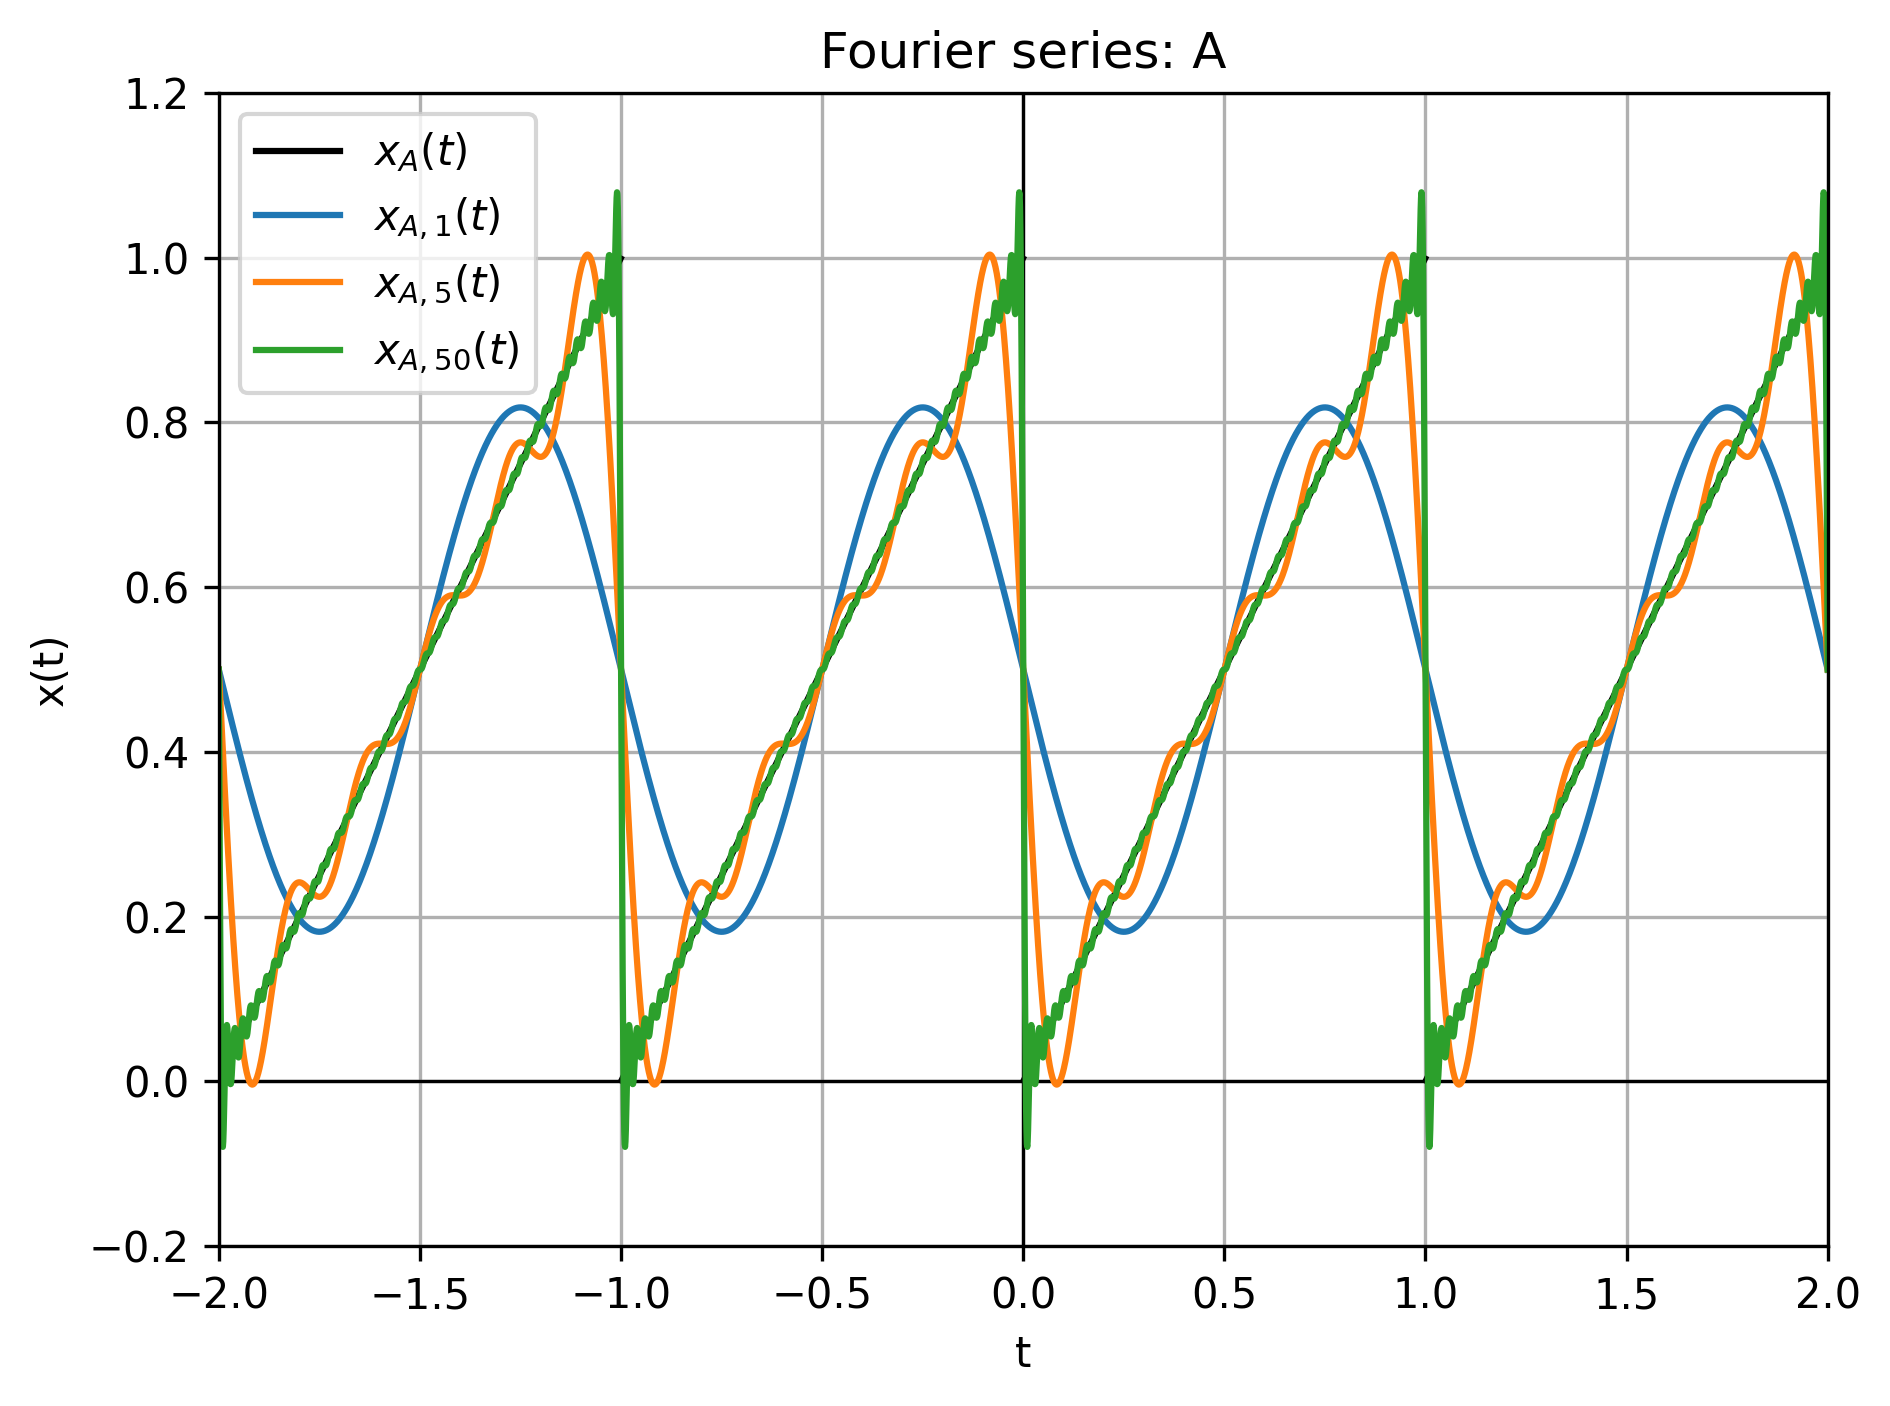
\includegraphics[width=0.9\textwidth]{../section4/kadai1_b_A.png}
  \caption{Aの元の関数と$M=1,5,50$のフーリエ部分和。}
  \label{fig:fourier-A}
\end{figure}

\begin{figure}[htbp]
  \centering
  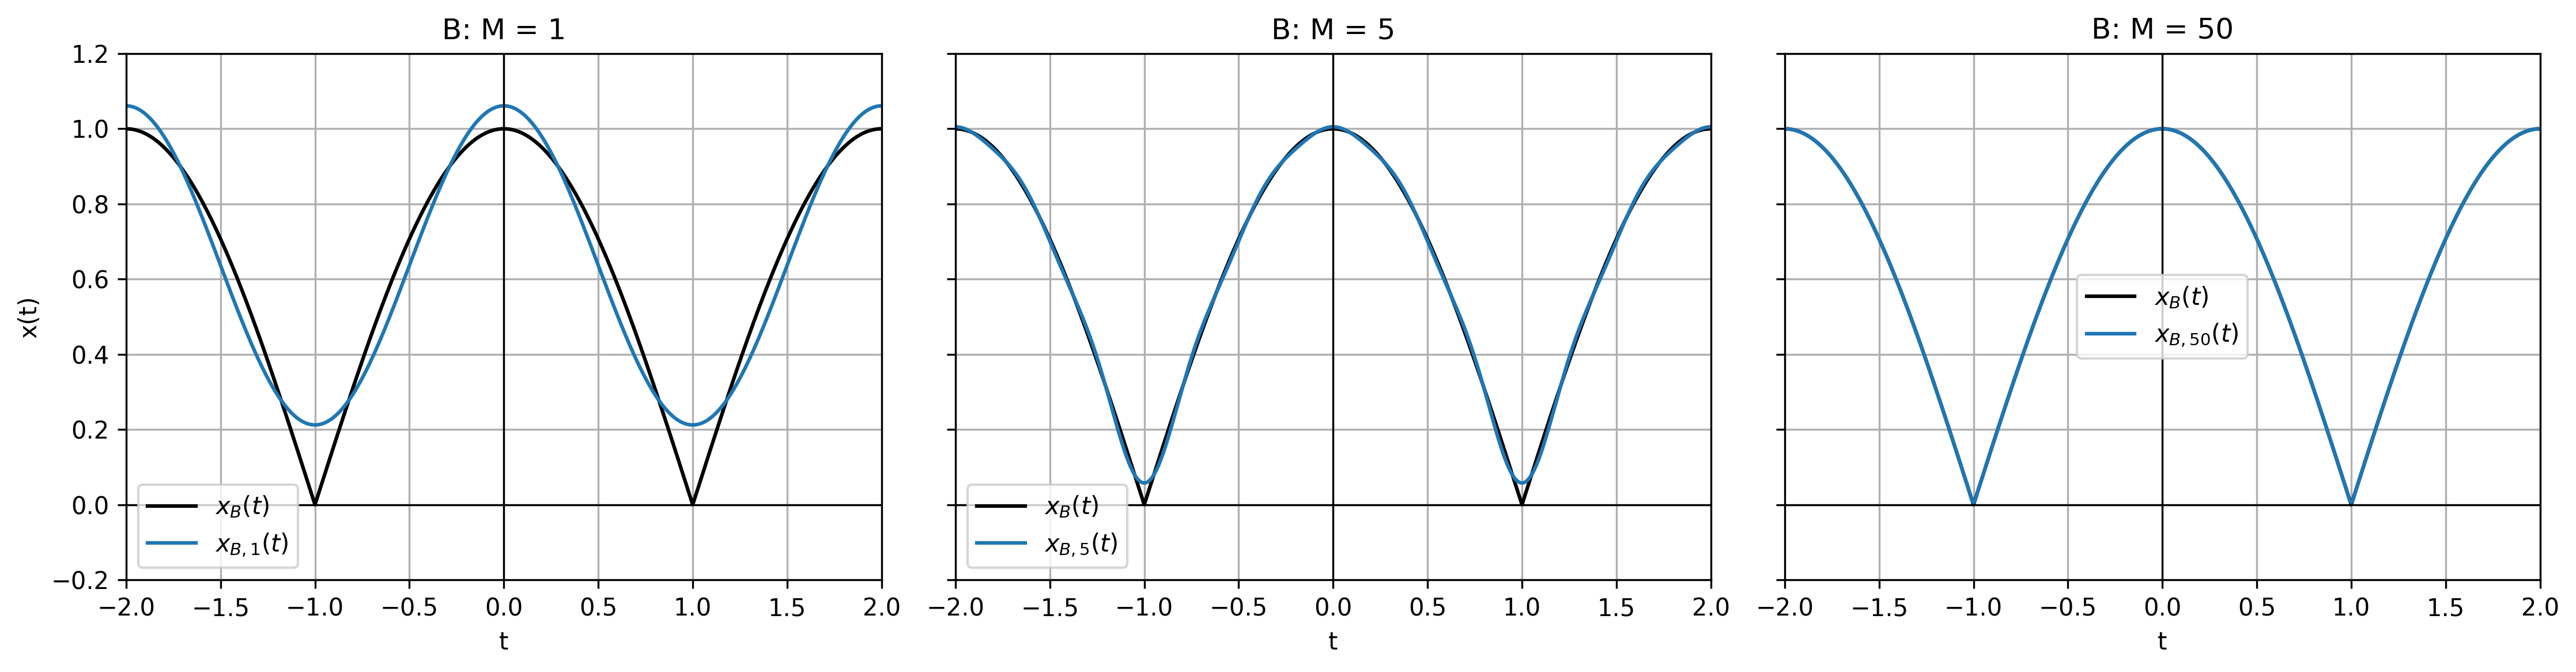
\includegraphics[width=0.9\textwidth]{../section4/kadai1_b_B.png}
  \caption{Bの元の関数と$M=1,5,50$のフーリエ部分和。}
  \label{fig:fourier-B}
\end{figure}

\subsubsection{問題(1-c)}

\begin{itembox}[l]{課題1-(c)}
上のA、Bの周期関数について、$M$を大きくしていったときの$x_M(t)$の収束の仕方の違いを比較し、その相違点を述べよ。
\end{itembox}

\subsubsection{実験方法(1-c)}

\subsubsection{結果(1-c)}

\subsubsection{考察(1-c)}

\subsection{問題2（動作テスト）}
\subsubsection{問題(2-a)}

\begin{itembox}[l]{問題2}
  次のような時系列データ $\{x_n\}_{n=0}^{7}$：
  \[
    \begin{aligned}
      x_0&=1, & x_1&=1, & x_2&=1, & x_3&=1,\\
      x_4&=0, & x_5&=0, & x_6&=0, & x_7&=0
    \end{aligned}
  \]
  が与えられたとき、以下の問いに答えよ。
  \begin{enumerate}
    \item[(a)] DFT［本文の式 (3.21)］の定義式に従ってフーリエ係数 $X_k$ を計算し、可能な限り厳密な形で求めよ。
  \end{enumerate}
\end{itembox}

\subsubsection{実験方法(2-a)}

本文の式は以下である。
\begin{equation}
  X_k=\sum_{n=0}^{N-1}x_n e^{-i\frac{2\pi kn}{N}},
  \tag{3.21}
  \label{eq:dft-definition}
\end{equation}
ここで$N=8$である。式変形を行い、以下に示す。

\subsubsection{結果(2-a)}

\[
  \begin{aligned}
    X_k
    &=\sum_{n=0}^{7}x_n e^{-i\frac{2\pi kn}{8}}\\
    &=x_0e^0+x_1e^{-i\frac{2\pi k}{8}}
      +x_2e^{-i\frac{4\pi k}{8}}+x_3e^{-i\frac{6\pi k}{8}}\\
    &=1+e^{-i\frac{\pi k}{4}}+e^{-i\frac{2\pi k}{4}}
      +e^{-i\frac{3\pi k}{4}}\\
    &=\sum_{n=0}^{3}\cos\left(\frac{nk\pi}{4}\right)
      -i\sum_{n=0}^{3}\sin\left(\frac{nk\pi}{4}\right).
  \end{aligned}
\]

ここで、$k=1,\ldots,7$について、
\[
  \begin{aligned}
    X_{N-k}=X_{8-k}
    &=\sum_{n=0}^{3}\cos\left(\frac{n(8-k)\pi}{4}\right)
      -i\sum_{n=0}^{3}\sin\left(\frac{n(8-k)\pi}{4}\right)\\
    &=\sum_{n=0}^{3}\cos\left(-\frac{nk\pi}{4}+2n\pi\right)
      -i\sum_{n=0}^{3}\sin\left(-\frac{nk\pi}{4}+2n\pi\right)\\
    &=\sum_{n=0}^{3}\cos\left(\frac{nk\pi}{4}\right)
      +i\sum_{n=0}^{3}\sin\left(\frac{nk\pi}{4}\right)\\
    &=\overline{X_k}.
  \end{aligned}
\]
よって、$k=0,1,2,3,4$を代入すれば、残りは共役対称性から求められる。

それぞれ代入すると、
\[
  \begin{aligned}
    X_0&=1+1+1+1=4,\\
    X_1&=1+\frac{1-i}{\sqrt{2}}-i+\frac{-1-i}{\sqrt{2}}
      =1-i(1+\sqrt{2}),\\
    X_2&=1-i-1+i=0,\\
    X_3&=1+\frac{-1-i}{\sqrt{2}}+i+\frac{1-i}{\sqrt{2}}
      =1-i(\sqrt{2}-1),\\
    X_4&=1-1+1-1=0.
  \end{aligned}
\]
共役対称性より、
\[
  \begin{aligned}
    X_5&=\overline{X_3}=1+i(\sqrt{2}-1),\\
    X_6&=\overline{X_2}=0,\\
    X_7&=\overline{X_1}=1+i(1+\sqrt{2}).
  \end{aligned}
\]

\subsubsection{考察(2-a)}

\subsubsection{問題(2-b)}

\begin{itembox}[l]{問題2-(b)}
FFTを用いてフーリエ係数 $X_k$ を数値的に求めよ。また、その結果 $(X_k^{\mathrm{FFT}})$ と (a)の結果 $(X_k^{\mathrm{exact}})$ との差から最大誤差
      \[
        \max_k\left|X_k^{\mathrm{FFT}}-X_k^{\mathrm{exact}}\right|
      \]
      を評価し、誤差の大きさを $10^{-K}$ のオーダーで表せ。さらに、誤差の原因について述べよ。
\end{itembox}

\begin{itembox}[l]{課題1-(b)}
二分法により関数 $f$ の全ての零点を求めよ。ただし、二つの異なる初期点は、(a)で描写した関数 $f$ の概形を参考にして適切に設定せよ。
\end{itembox}
\paragraph{二分法の実装と条件}

\texttt{kadai1\_b.py}から\texttt{bisection}を呼び出した。(a)で描画したグラフの三つの交点をそれぞれ含む区間$[-5,-2.5]$、$[-2.5,0]$、$[0,2.5]$を選んだ。端点の関数値は順に$(-56,3.375)$、$(3.375,-6)$、$(-6,9.625)$であり、各区間で符号が異なる。実装では負の関数値を持つ端点を$a$、非負の関数値を持つ端点を$b$として保持するため、数値として$a<b$とは限らない。中点$c=(a+b)/2$を計算し、$f(c)$の符号に応じて同符号の端点を$c$へ置き換える。

\par\noindent
コード\ref{lst:bisection}に、\texttt{utils\_math.py}の14〜34行を示す。
\par
\lstinputlisting[firstline=14,lastline=34,firstnumber=14,language=Python,caption={課題1-(b)の二分法},label={lst:bisection}]{../section3/utils_math.py}


\par\noindent
コード\ref{lst:bisect-call}に、\texttt{kadai1\_b.py}の全体を示す。
\par
\lstinputlisting[language=Python,firstnumber=1,caption={課題1-(b)の初期区間},label={lst:bisect-call}]{../section3/kadai1_b.py}



\begin{itembox}[l]{課題1-(c)}
ニュートン法により関数 $f$ の全ての零点を求めよ。ただし、(a)で描写した関数 $f$ の概形を参考にして、零点の近くに初期点を設定せよ。
\end{itembox}
\paragraph{ニュートン法}

\texttt{kadai1\_c.py}で、(a)で描画したグラフの交点を参考に初期点$-2.5,0,2.5$を選んだ。\texttt{newton}は$f'(x)=3x^2+4x-5$を用い、
\begin{align}
  x^{k+1}=x^k-\frac{f(x^k)}{f'(x^k)}
  \label{eq:root-newton}
\end{align}
と更新する。

\par\noindent
コード\ref{lst:root-newton}に、\texttt{utils\_math.py}の38〜54行を示す。
\par
\lstinputlisting[firstline=38,lastline=54,firstnumber=38,language=Python,caption={課題1-(c)のニュートン法},label={lst:root-newton}]{../section3/utils_math.py}



\par\noindent
コード\ref{lst:root-newton-call}に、\texttt{kadai1\_c.py}の全体を示す。
\par
\lstinputlisting[language=Python,firstnumber=1,caption={課題1-(c)の初期点},label={lst:root-newton-call}]{../section3/kadai1_c.py}

\subsection{課題1：関数の零点探索}

\begin{figure}[htbp]
  \centering
  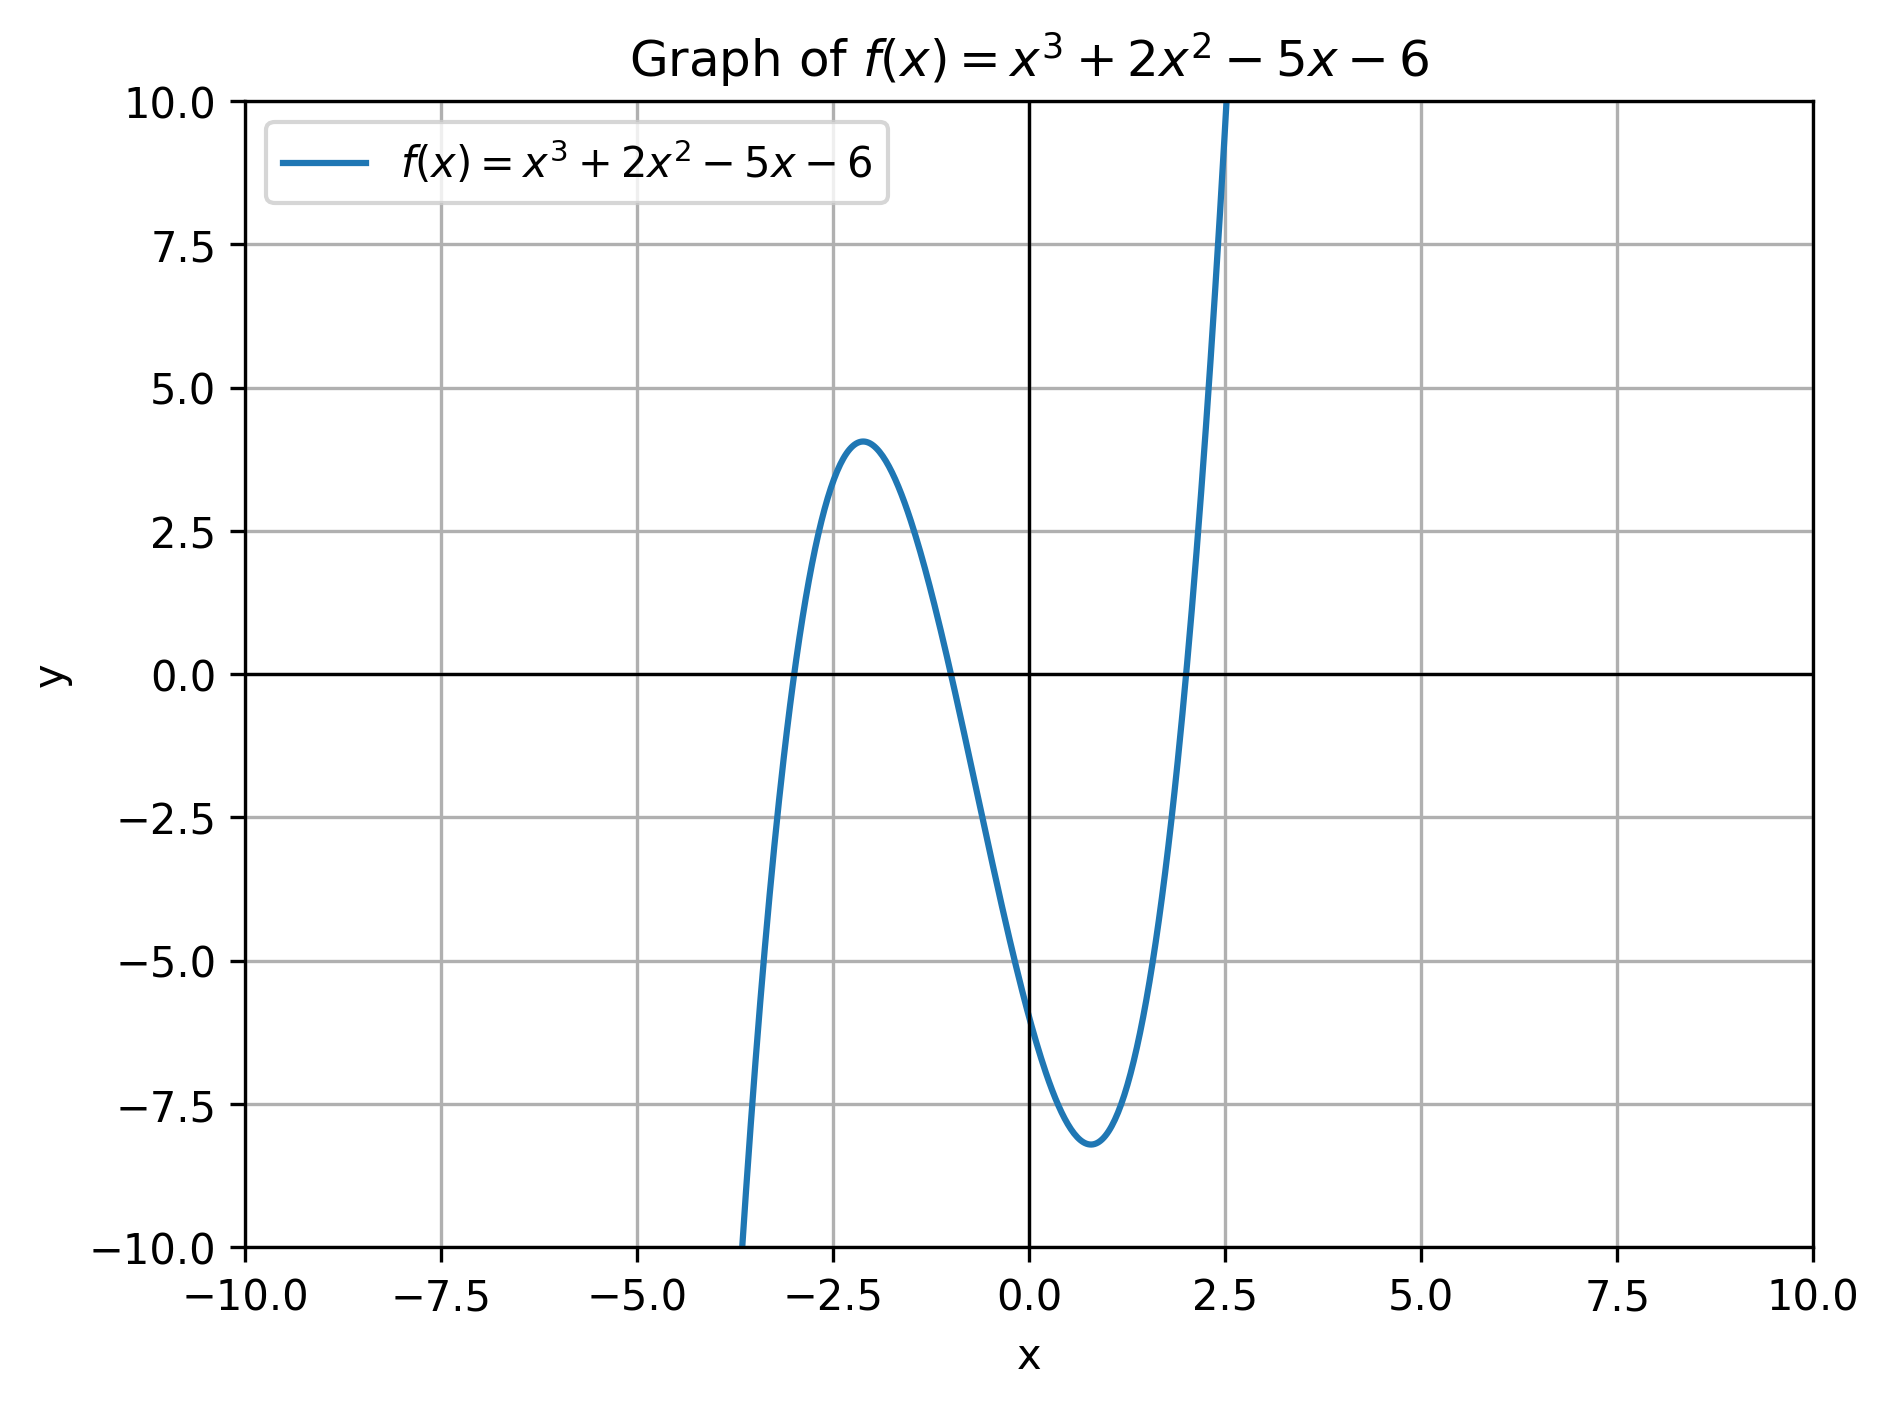
\includegraphics[width=0.8\linewidth]{../section3/kadai1_a.png}
  \caption{課題 1-(a)の描画結果。}
  \label{fig:example}
\end{figure}

\paragraph{二分法}
二分法で求めた零点の近似値は、約$-3$、$-1$、$2$であった。各初期区間に対する近似値は表\ref{tab:bisect}の通りであり、この結果は\texttt{kadai1\_b.txt}に保存されている。
\begin{table}[htbp]
  \centering
  \caption{二分法の結果。}
  \label{tab:bisect}
  \begin{tabular}{lr}\hline
    初期区間 & 零点の近似値\\\hline
    $[-5,-2.5]$ & $-2.9999999999999716$\\
    $[-2.5,0]$ & $-0.9999999999999432$\\
    $[0,2.5]$ & $2.0000000000000284$\\\hline
  \end{tabular}
\end{table}

\paragraph{ニュートン法}
ニュートン法で求めた零点の近似値は、$-3.0$、$-1.0$、$2.0$であった。各初期点に対する近似値は表\ref{tab:root-newton}の通りであり、この結果は\texttt{kadai1\_c.txt}に保存されている。
\begin{table}[htbp]
  \centering
  \caption{零点探索のニュートン法の結果。}
  \label{tab:root-newton}
  \begin{tabular}{rr}\hline
    初期点 & 得られた点\\\hline
    $-2.5$ & $-3.0$\\
    $0$ & $-1.0$\\
    $2.5$ & $2.0$\\\hline
  \end{tabular}
\end{table}

零点探索と最適化の方法をPythonで実装し、得られた値や更新回数を比較した。零点探索では、二分法とニュートン法のどちらでも、$-3$、$-1$、$2$に近い値が得られた。1変数の最適化でも、最急降下法とニュートン法でともに$x=3$に近い値が得られた。

\subsubsection{実験方法(2-b)}
以下のように式を変形し、アルゴリズムを考える。

$W_N=e^{-i2\pi/N}$とおく。$N=8$として、偶数番目と奇数番目の項に分けると、
\[
  \begin{aligned}
    X_k
    &=\sum_{n=0}^{7}x_n e^{-i\frac{2\pi kn}{8}}
      =\sum_{n=0}^{7}x_n(W_8)^{kn}\\
    &=x_0+x_1(W_8)^k+x_2(W_8)^{2k}+x_3(W_8)^{3k}\\
    &\quad+x_4(W_8)^{4k}+x_5(W_8)^{5k}
      +x_6(W_8)^{6k}+x_7(W_8)^{7k}\\
    &=\sum_{m=0}^{3}x_{2m}(W_8)^{2mk}
      +\sum_{m=0}^{3}x_{2m+1}(W_8)^{(2m+1)k}\\
    &=\sum_{m=0}^{3}x_{2m}(W_4)^{mk}
      +(W_8)^k\sum_{m=0}^{3}x_{2m+1}(W_4)^{mk}\\
    &=X_k^{(0)}+(W_8)^kX_k^{(1)}.
  \end{aligned}
\]
ここで、
\[
  X_k^{(0)}=\sum_{m=0}^{3}x_{2m}(W_4)^{mk},\qquad
  X_k^{(1)}=\sum_{m=0}^{3}x_{2m+1}(W_4)^{mk}
\]
であり、$(W_8)^{2mk}=(W_4)^{mk}$を用いた。

また、$a=0,1$について、
\[
  \begin{aligned}
    X_{k+4}^{(a)}
    &=\sum_{m=0}^{3}x_{2m+a}(W_4)^{m(k+4)}\\
    &=\sum_{m=0}^{3}x_{2m+a}(W_4)^{mk}e^{-i2\pi m}
      =X_k^{(a)},\\
    (W_8)^{k+4}
    &=e^{-i\pi}(W_8)^k=-(W_8)^k.
  \end{aligned}
\]
よって、$k=0,1,2,3$について、
\[
  \begin{aligned}
    X_k&=X_k^{(0)}+(W_8)^kX_k^{(1)},\\
    X_{k+4}&=X_k^{(0)}-(W_8)^kX_k^{(1)}.
  \end{aligned}
\]

さらに、各項を同様に分ける。
\[
  \begin{aligned}
    X_k
    &=\bigl(x_0+x_2(W_8)^{2k}+x_4(W_8)^{4k}+x_6(W_8)^{6k}\bigr)\\
    &\quad+\bigl(x_1(W_8)^k+x_3(W_8)^{3k}
      +x_5(W_8)^{5k}+x_7(W_8)^{7k}\bigr)\\
    &=\bigl(x_{2\cdot0}+x_{2\cdot1}(W_8)^{2k}
      +x_{2\cdot2}(W_8)^{4k}+x_{2\cdot3}(W_8)^{6k}\bigr)\\
    &\quad+\bigl(x_{2\cdot0+1}(W_8)^k+x_{2\cdot1+1}(W_8)^{3k}\\
    &\qquad\qquad+x_{2\cdot2+1}(W_8)^{5k}
      +x_{2\cdot3+1}(W_8)^{7k}\bigr)\\
    &=\bigl(x_{2\cdot0}+x_{2\cdot2}(W_8)^{4k}\bigr)
      +\bigl(x_{2\cdot1}(W_8)^{2k}+x_{2\cdot3}(W_8)^{6k}\bigr)\\
    &\quad+\bigl(x_{2\cdot0+1}(W_8)^k+x_{2\cdot2+1}(W_8)^{5k}\bigr)\\
    &\quad+\bigl(x_{2\cdot1+1}(W_8)^{3k}+x_{2\cdot3+1}(W_8)^{7k}\bigr)\\
    &=\sum_{m=0}^{1}x_{2(2m+0)+0}(W_2)^{mk}
      +(W_4)^k\sum_{m=0}^{1}x_{2(2m+1)+0}(W_2)^{mk}\\
    &\quad+(W_8)^k\Bigl\{
      \sum_{m=0}^{1}x_{2(2m+0)+1}(W_2)^{mk}\\
    &\qquad\qquad+(W_4)^k\sum_{m=0}^{1}x_{2(2m+1)+1}(W_2)^{mk}\Bigr\}\\
    &=X_k^{(00)}+(W_4)^kX_k^{(01)}
      +(W_8)^k\left\{X_k^{(10)}+(W_4)^kX_k^{(11)}\right\}.
  \end{aligned}
\]
ここで、$a,b=0,1$として、
\[
  X_k^{(ab)}=\sum_{m=0}^{1}x_{2(2m+b)+a}(W_2)^{mk}
\]
とした。もう一度分けると、
\[
  \begin{aligned}
    X_k
    &=X_k^{(000)}+(W_2)^kX_k^{(001)}\\
    &\quad+(W_4)^k\left\{X_k^{(010)}+(W_2)^kX_k^{(011)}\right\}\\
    &\quad+(W_8)^k\Bigl[
      X_k^{(100)}+(W_2)^kX_k^{(101)}\\
    &\qquad\qquad+(W_4)^k\left\{X_k^{(110)}+(W_2)^kX_k^{(111)}\right\}
      \Bigr].
  \end{aligned}
\]
ここで、$a,b,c=0,1$について、
\[
  \begin{aligned}
    X_k^{(abc)}
    &=\sum_{m=0}^{8/8-1}x_{2^3m+2^2c+2^1b+2^0a}(W_1)^{mk}\\
    &=x_{2^2c+2^1b+2^0a}=x_{(cba)_2}.
  \end{aligned}
\]
したがって、$X_k^{(abc)}$は$k$によらない。

\subsubsection{結果(2-b)}
FFTで求めたフーリエ係数は次のとおりであった。
\[
  \begin{aligned}
    X_0&=4,\\
    X_1&=1-2.414213562373095i,\\
    X_2&=0,\\
    X_3&=1-0.4142135623730949i,\\
    X_4&=0,\\
    X_5&=1+0.4142135623730949i,\\
    X_6&=0,\\
    X_7&=1+2.414213562373095i.
  \end{aligned}
\]
最大誤差は
\[
  \max_k\left|X_k^{\mathrm{FFT}}-X_k^{\mathrm{exact}}\right|
  =2.220446049250313\times10^{-16}
\]
であり、$K=15.653559774527022$であった。したがって、誤差の大きさは$10^{-16}$程度であった。

\paragraph{生成AIの利用}
課題6-2,3の調査・理解の中でOpenAI Codexを利用した。

\begin{thebibliography}{9}

\end{thebibliography}

\end{document}
